\chapter{Testing}
The reason behind testing was to find errors. Every program or software has errors in it, against the common view that there are no errors in it if the program or softare is working executing the programs with the intention of finding the errors in it is therefore testing; hence a successful test is one which finds errors. Testing is an activity however, it is restricted to being performed after the development phase is complete, but is carried paraller with all stages of system development, starting with requirement specificaton.

Test cases were devised with a purpose in mind. A test case is a set of data that a system will process as normal input. The software units developed in the system are modules and routines that are assembled and integrated to perform the required function of the system. Test results once gathered and evaluted, provide a qualitative indication of the software quality and reliability and serve as the basis for design modification if required. In this phase, testing is done at different levels. Actually testing phase of the implementations works accurately and efficently before live operation commences.

The primary objective of testing includes:-
\begin{itemize}
	\item To identify defects in the application.
	\item The most important role of testing is simply to provide information.
	\item To check the proper working of the application while CRUD functions works properly.
\end{itemize}

  
\section{Functional Tests}

\subsection{Acceptance Tests}

Acceptance tests are ensuring that the main requirements agreed for the project are met in the current version. So they need to prove that it is possible for a user to achieve at least the main goals for which he is using the web application, reason why they will be covering the top-level use cases described in the early section Use Case Model. Given that acceptance tests are guaranteeing the correctness of the current version, it is imperative to use real data instead of mocking it.

These type of tests need to be supervised by the client of the product, usually non-technical people. This makes it a requirement to be easy to understand them by using a plain language to define the rules. Cucumber is used in this project as a tool to write these acceptance tests, allowing to write the rules in plain text (see Figure 6.5), while describing the technical details of each rule in Ruby in a separated file.

\begin{figure}[!h]
\center
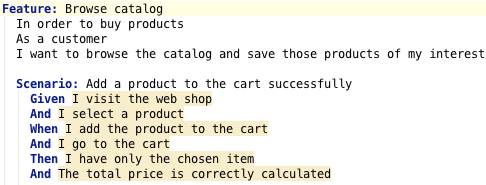
\includegraphics[keepaspectratio, width=12cm]{images/browse-catalog-testing-rules.png}
\caption{Example of rules to verify that browsing catalog can be achieved, in browseCatalog.feature- Guya E-commerce}
\end{figure}


\section{Performance Tests}

Constantly during the project development, the tool Chrome DevTools was used to check the performance of the projects web, paying special attention to repeated calls or some unexpected behavior resulting from a flaw in the software. This way it was possible to detect a bug in the endless scroll for the product list, which executed repeated calls to the web application server even when there were no more product available. Also some methods with high response times could be fine-tuned with this tool.

Another tool from Google, PageSpeed Insights, is an online performance test that analyzes the web page looking for elements that may affect its fast execution, such as resources that may unnecessary block the page. This test suggested to use minified versions of the JavaScript and CSS files, which was an easy task thanks to Webpack compiler built-in support.

It also reported that there were too many JavaScript and CSS files being fetched before the page could even be loaded, which meant that the browser had to wait until the last file was fetched in order to allow the user take control of it. It was necessary to find a solution for this, because in order to make the system’s Reactjs components more understandable for the developer, the code was split into several files and classes, which in some cases raised the amount of files fetched to more than ten.

The best way to face this issue was to use RequireJS, an asynchronously module and file loader for JavaScript files, that allowed to fetch a JavaScript file in the background first, and then load all its dependencies in parallel. Although it required a bit of effort to integrate with the current code, the results were very satisfactory. It is also worth mentioning that almost all third-party client-side libraries are being fetched from CDNJS, a community-driven CDN\footnote{CDN stands for Content Management Network and it is a large distributed system of servers deployed in multiple data centers across the Internet, allowing to server content with high availability and performance.} for web libraries that allows to decrease the loading time considerably.